\documentclass[11pt]{article}
\usepackage{amssymb, amsmath}
\usepackage{amsthm}
\usepackage{url,hyperref}
\usepackage{algorithm}
\usepackage{algpseudocode}
\usepackage[numbered]{mcode}
\usepackage{graphicx}

\topmargin -2cm
\textheight 23cm
\textwidth 6.5in
\oddsidemargin -.1in
\evensidemargin -.1in
\topmargin -1.5cm
\linespread{1.25}

% ----------------------------------------------------------------
% TODO: Enter your name, and your student number, and your topic below
% ----------------------------------------------------------------
\newcommand{\SName}{{Gabriel Luong}}
\newcommand{\SNumber}{{996268275}}
\newcommand{\Topic}{{CSC420 Assignment 2}}
% ----------------------------------------------------------------

\title{\Topic\\
}
\author{
	\SName \\ 
	\SNumber 
	\date{}
}

\begin{document}
\maketitle
%----------------------------------------------------------------
% Question 1
%----------------------------------------------------------------
\section{}
\begin{lstlisting}
% Given an image, perform Harris corner detection and return the result image
function harris(im)
img = rgb2gray(im);

[Ix, Iy] = imgradientxy(img); % Compute the gradients Ix and Iy
Ix2 = Ix.^2;
Iy2 = Iy.^2;
Ixy = Ix.*Iy;

% Convolve the computed gradients with a Gaussian filter
gaussian = fspecial('gaussian');
gIx2 = imfilter(Ix2, gaussian, 'same', 'conv');
gIy2 = imfilter(Iy2, gaussian, 'same', 'conv');
gIxy = imfilter(Ixy, gaussian, 'same', 'conv');

height = size(im, 1);
width = size(im, 2);
alpha = 0.06;
R = zeros(height, width);

% Compute M and R for every pixel
for i = 1:height
    for j = 1:width
        M = [gIx2(i, j) gIxy(i, j); ...
             gIxy(i, j) gIy2(i, j)];
        detM = (gIx2(i, j) * gIy2(i, j)) - gIxy(i, j)^2;
        traceM = gIx2(i, j) + gIy2(i, j);
        R(i, j) = detM - (alpha * traceM ^ 2);
    end
end

% Keep track of the points to plot
X = [];
Y = [];

threshold = max(max(R)) * 0.03; % R threshold

% Perform non-maximum suppression by checking surrounding R values for a
% local maxima with a radius of 1
for i = 2:height - 1
    for j = 2:width - 1
        if R(i, j) > threshold && R(i, j) > R(i - 1, j + 1) && R(i, j) > R(i, j + 1) &&
        	  	R(i, j) > R(i + 1, j + 1) && R(i, j) > R(i - 1, j) && R(i, j) > R(i + 1, j) &&
			R(i, j) > R(i - 1, j - 1) && R(i, j) > R(i, j - 1) && R(i, j) > R(i - 1, j + 1)
            X(end+1) = j;
            Y(end+1) = i;
        end
    end
end

% Display the results of the computations
figure, imshow(Ix, []), title('Ix')
figure, imshow(Iy, []), title('Iy')
figure, imshow(Ix2, []), title('Ix2')
figure, imshow(Iy2, []), title('Iy2')
figure, imshow(Ixy, []), title('Ixy')
figure, imshow(gIx2, []), title('gIx2')
figure, imshow(gIy2, []), title('gIy2')
figure, imshow(gIxy, []), title('gIxy')
figure, imshow(R, []), title('R');
figure, imshow(img), title('corners');
hold on;
plot(X, Y, 'R+');
end
\end{lstlisting}
(a) Compute $I_{x}^{2}$, $I_{y}^{2}$, $I_{x}I_{y}$ and the matrix M for every pixel.
\begin{lstlisting}
img = rgb2gray(im);

[Ix, Iy] = imgradientxy(img); % Compute the gradients Ix and Iy
Ix2 = Ix.^2;
Iy2 = Iy.^2;
Ixy = Ix.*Iy;

% Convolve the computed gradients with a Gaussian filter
gaussian = fspecial('gaussian');
gIx2 = imfilter(Ix2, gaussian, 'same', 'conv');
gIy2 = imfilter(Iy2, gaussian, 'same', 'conv');
gIxy = imfilter(Ixy, gaussian, 'same', 'conv');

height = size(im, 1);
width = size(im, 2);
alpha = 0.06;
R = zeros(height, width);

% Compute M and R for every pixel
for i = 1:height
    for j = 1:width
        M = [gIx2(i, j) gIxy(i, j); gIxy(i, j) gIy2(i, j)];
    end
end
\end{lstlisting}
(b) Given the matrix A = $\bigl(\begin{smallmatrix} a&b\\ c&d \end{smallmatrix} \bigr)$, the determinant $det(A) = ad - cb$, and $trace(A) = a + d$. The equation to compute the cornerness measure R in each pixel is $R = det(M) - \alpha trace(M)^2 = ad - cb - \alpha (a + d)^2$.
\\\\
(c) Compute R for every pixel.
\begin{lstlisting}
% Convolve the computed gradients with a Gaussian filter
gaussian = fspecial('gaussian');
gIx2 = imfilter(Ix2, gaussian, 'same', 'conv');
gIy2 = imfilter(Iy2, gaussian, 'same', 'conv');
gIxy = imfilter(Ixy, gaussian, 'same', 'conv');

height = size(im, 1);
width = size(im, 2);
alpha = 0.06;
R = zeros(height, width);

% Compute M and R for every pixel
for i = 1:height
    for j = 1:width
        M = [gIx2(i, j) gIxy(i, j); ...
             gIxy(i, j) gIy2(i, j)];
        detM = (gIx2(i, j) * gIy2(i, j)) - gIxy(i, j)^2;
        traceM = gIx2(i, j) + gIy2(i, j);
        R(i, j) = detM - (alpha * traceM ^ 2);
    end
end
\end{lstlisting}
(d) Compute Threshold R and perform non-maxima suppression.
\begin{lstlisting}
% Keep track of the points to plot
X = [];
Y = [];

threshold = max(max(R)) * 0.03; % R threshold

% Perform non-maximum suppression by checking surrounding R values for a
% local maxima with a radius of 1
for i = 2:height - 1
    for j = 2:width - 1
        if R(i, j) > threshold && R(i, j) > R(i - 1, j + 1) && R(i, j) > R(i, j + 1) &&
        	  	R(i, j) > R(i + 1, j + 1) && R(i, j) > R(i - 1, j) && R(i, j) > R(i + 1, j) &&
			R(i, j) > R(i - 1, j - 1) && R(i, j) > R(i, j - 1) && R(i, j) > R(i - 1, j + 1)
            X(end+1) = j;
            Y(end+1) = i;
        end
    end
end

figure, imshow(img), title('corners');
hold on;
plot(X, Y, 'R+');
\end{lstlisting}
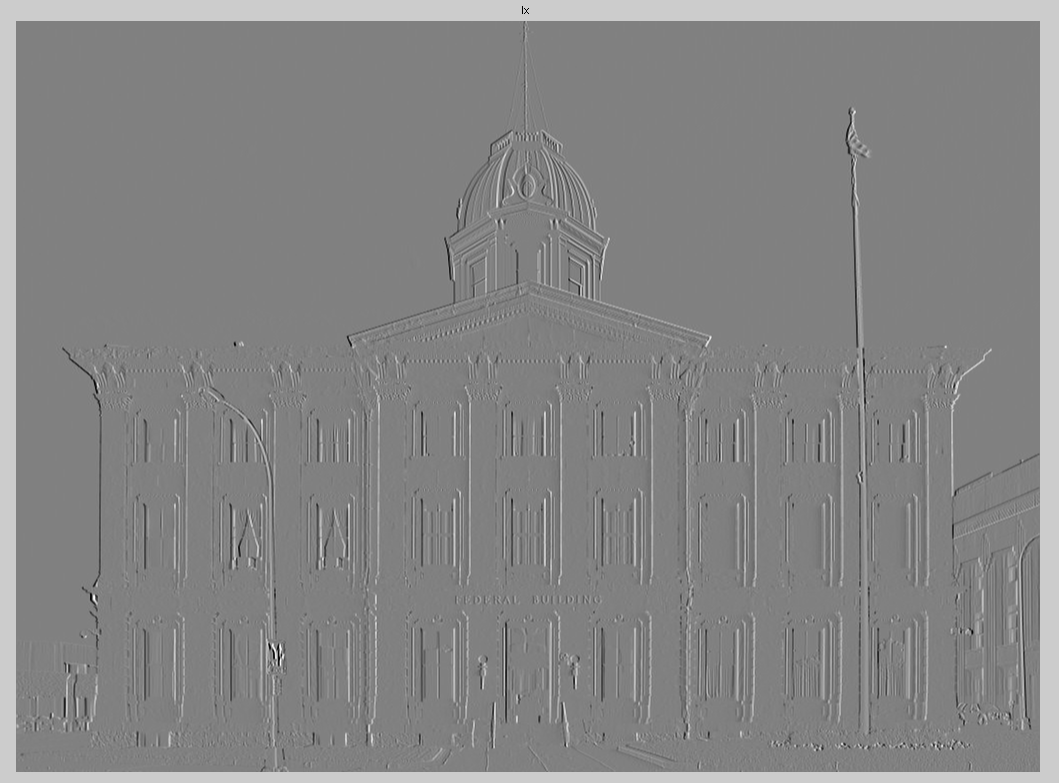
\includegraphics[scale=0.5]{lx}
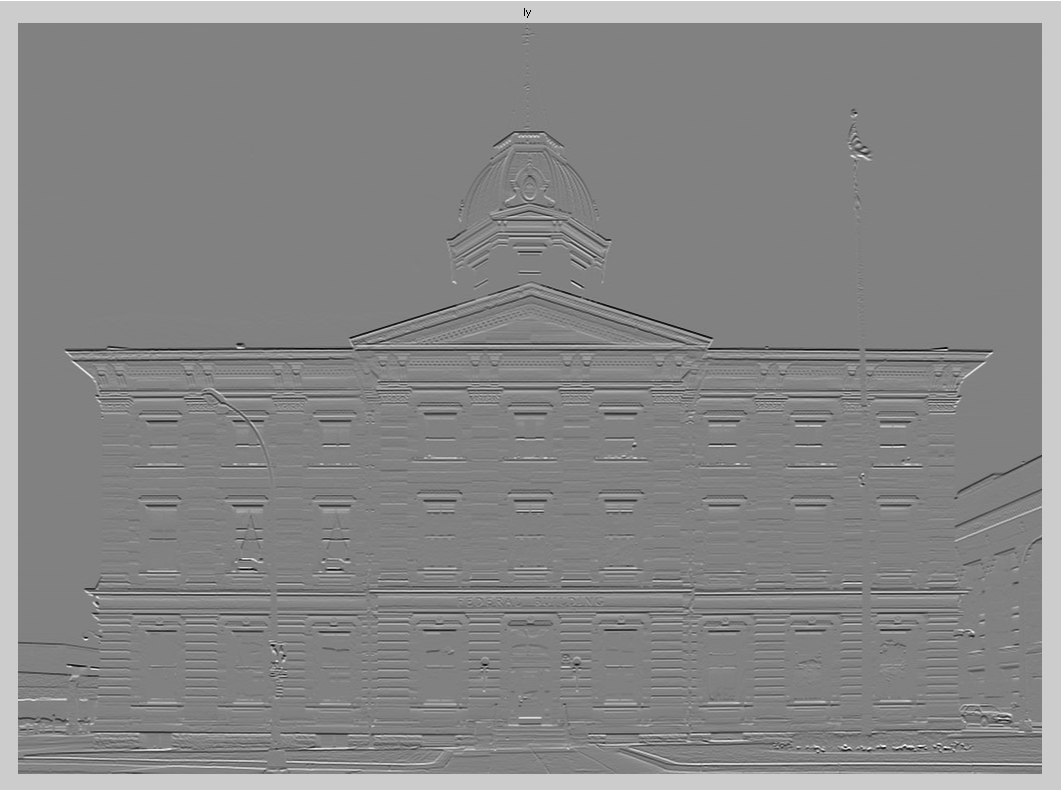
\includegraphics[scale=0.5]{Iy}
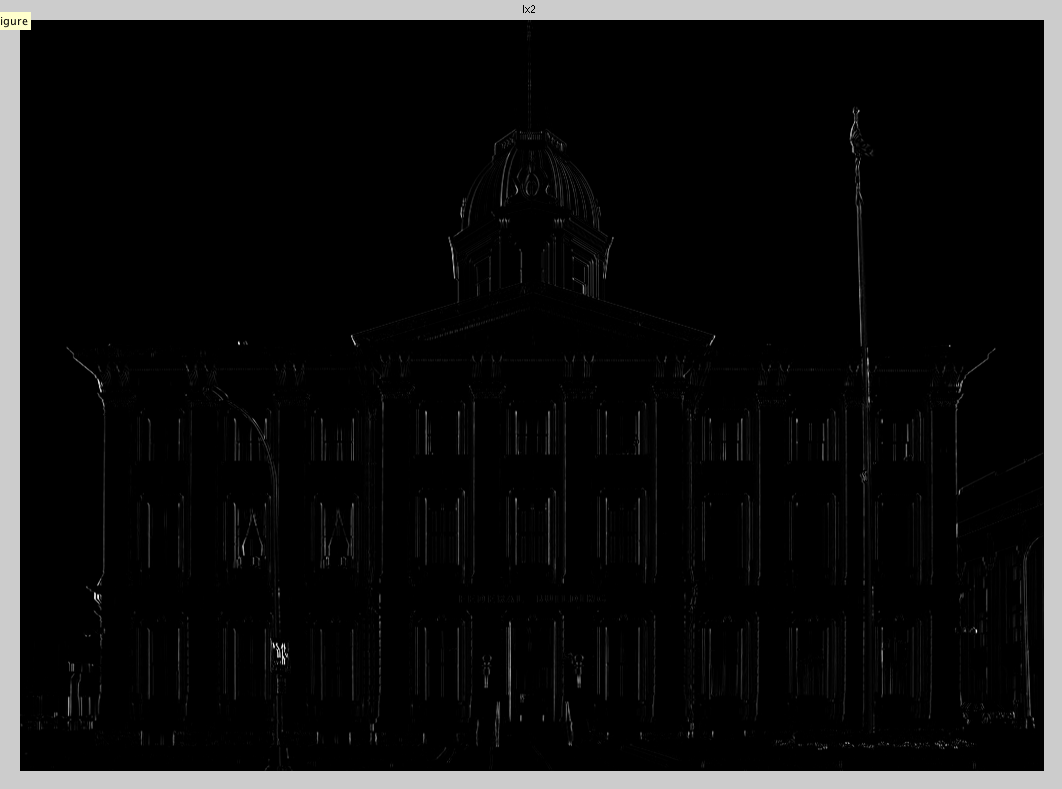
\includegraphics[scale=0.5]{Ix2}
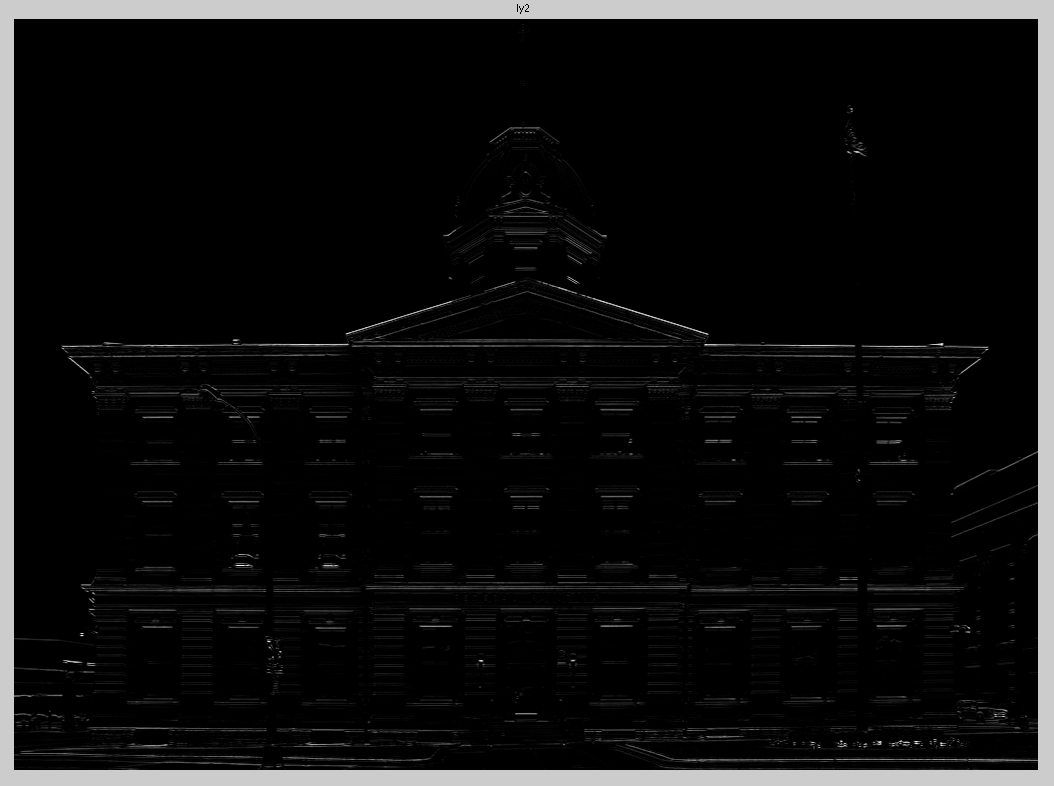
\includegraphics[scale=0.5]{Iy2}
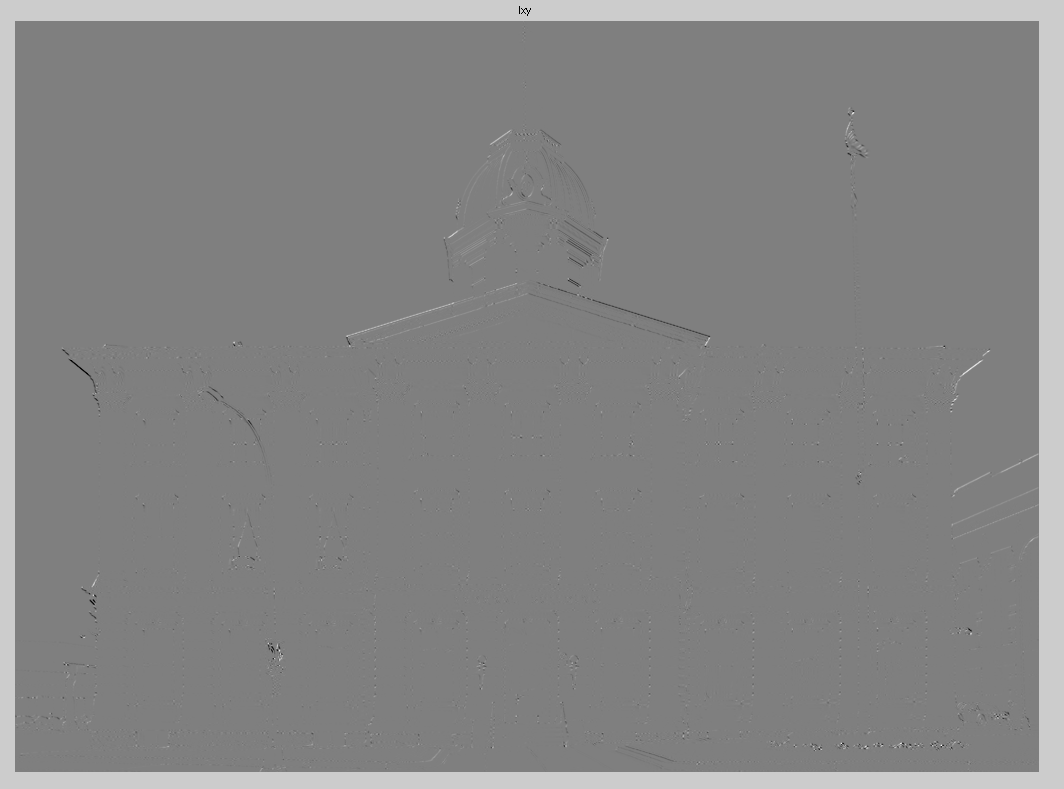
\includegraphics[scale=0.5]{Ixy}
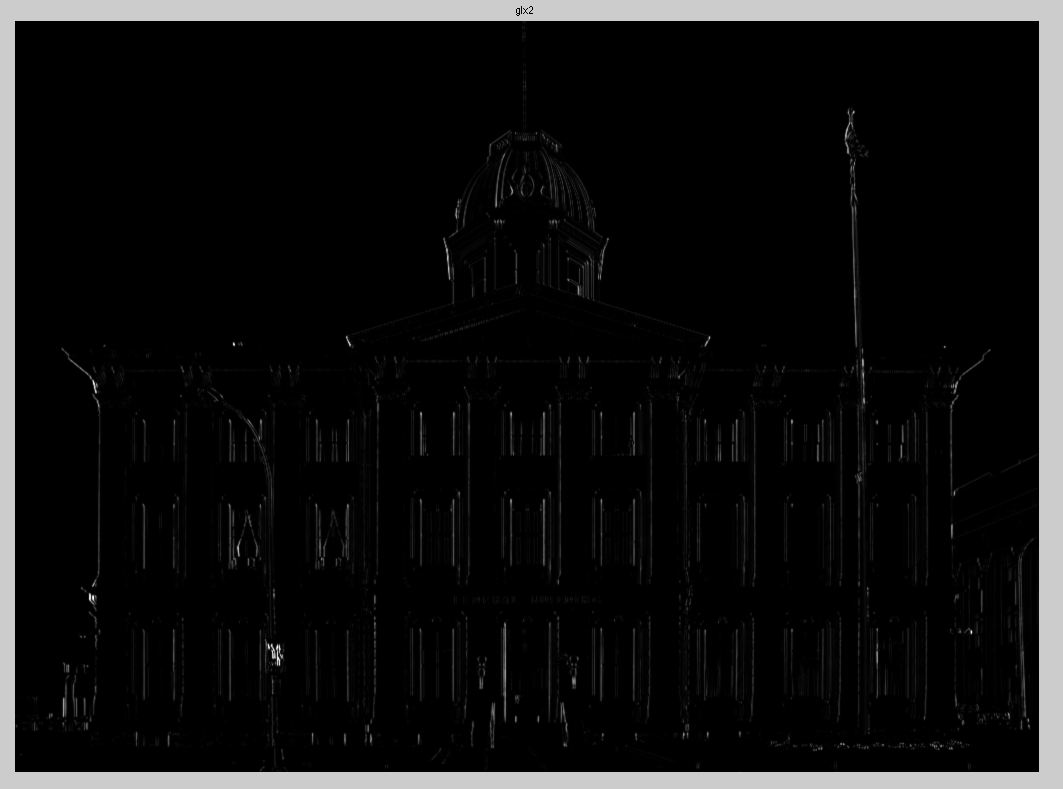
\includegraphics[scale=0.5]{glx2}
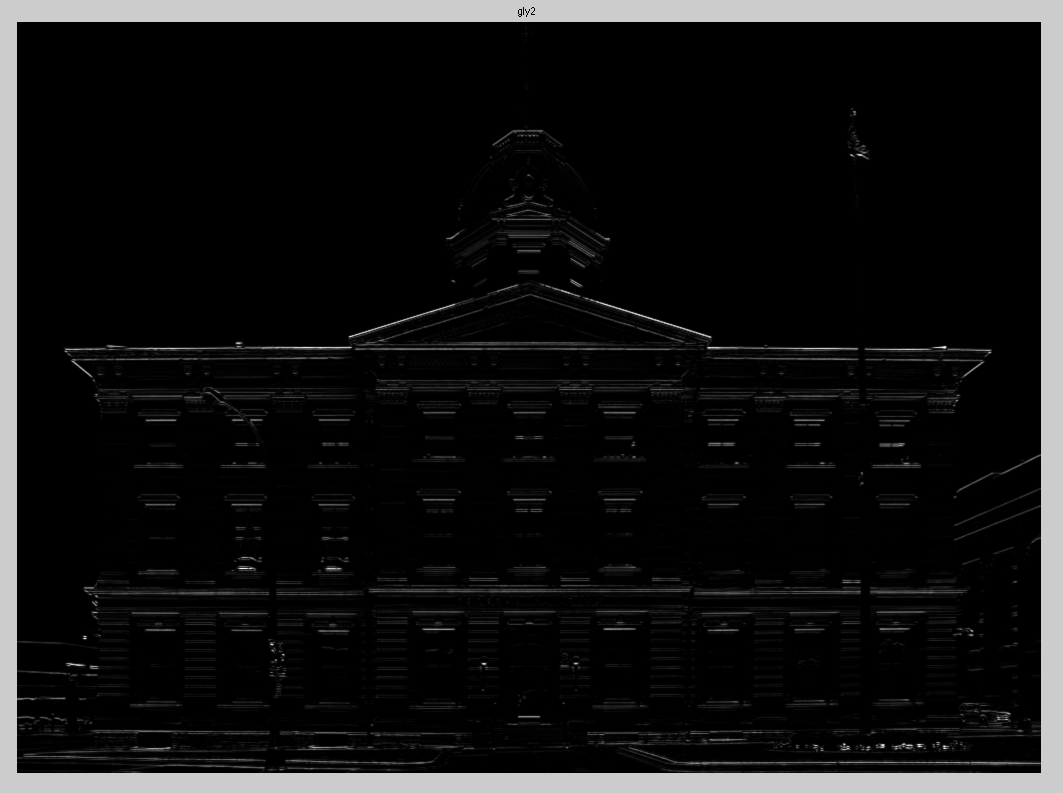
\includegraphics[scale=0.5]{gly2}
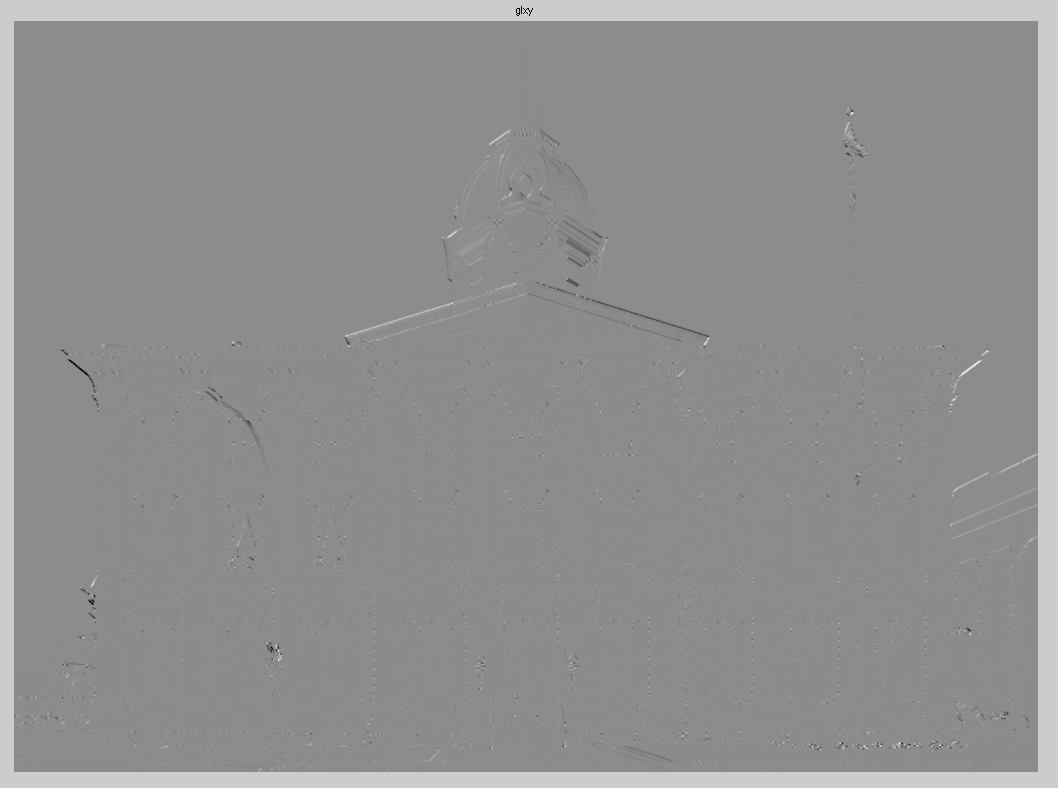
\includegraphics[scale=0.5]{glxy}
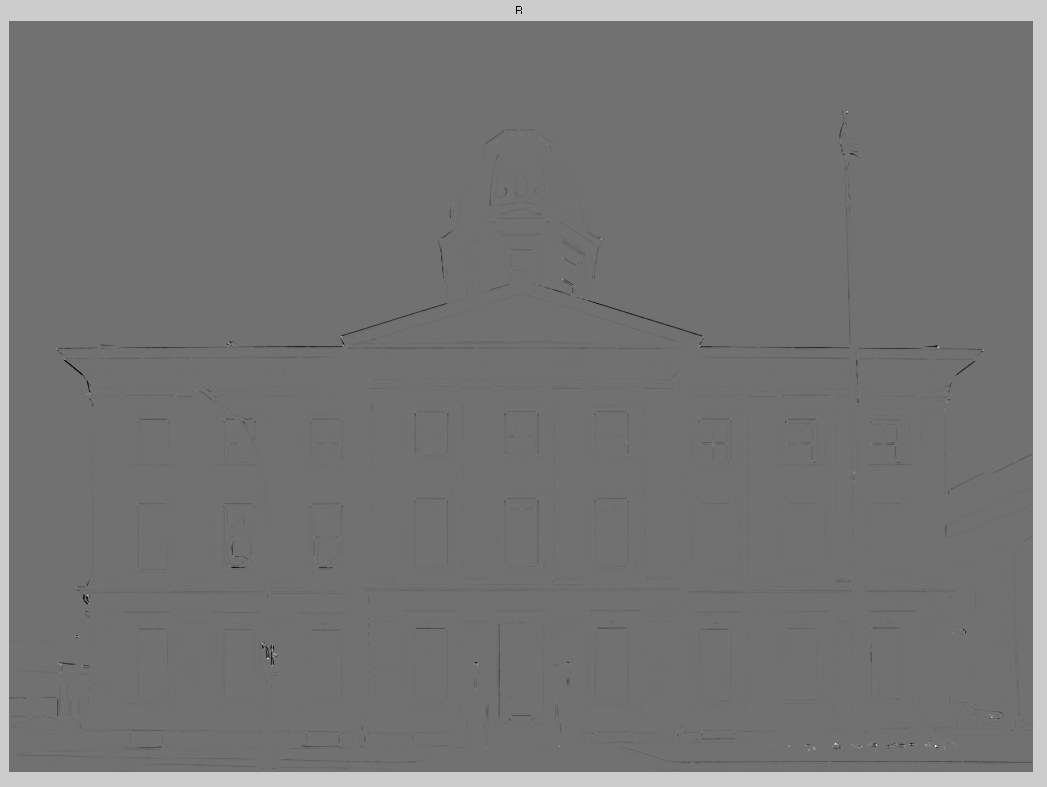
\includegraphics[scale=0.5]{R}
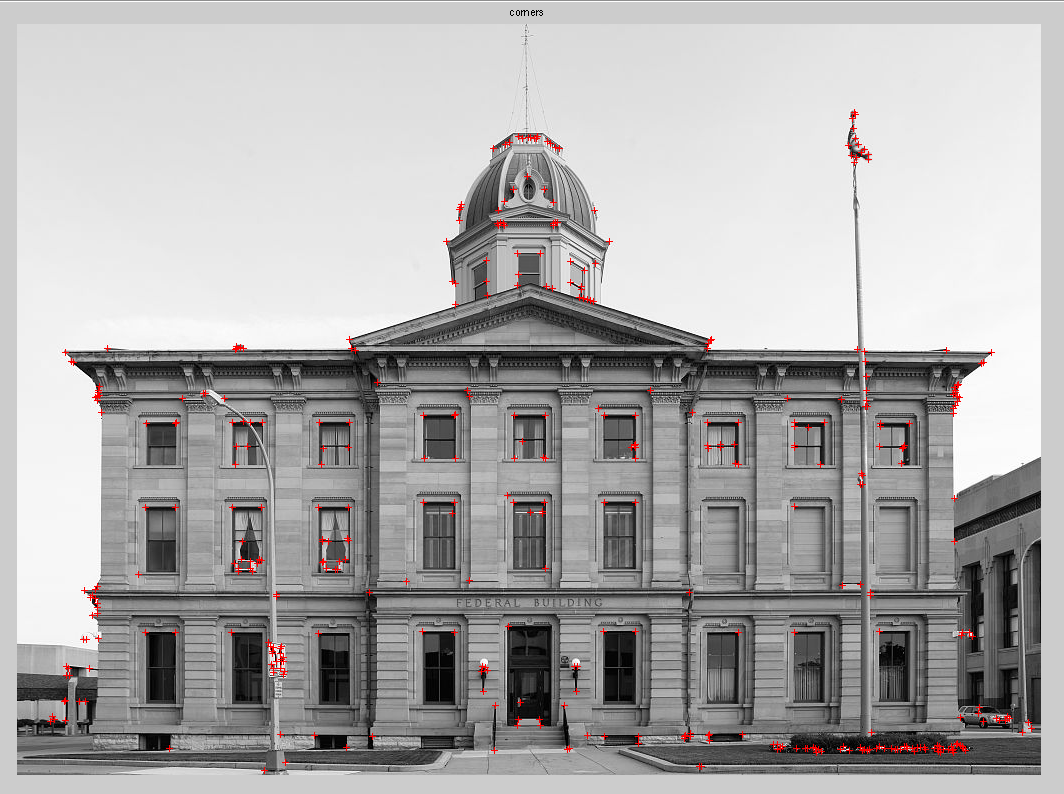
\includegraphics[scale=0.5]{corners}
%----------------------------------------------------------------
% Question 2
%----------------------------------------------------------------
\section{}

\end{document}